\section{Experimental Setup}
\label{sec:experiment}
%
In this section, we present the setup of our experiments to evaluate
the effectiveness of \tool. We answer the following research
questions (RQs):

\begin{enumerate}[label=\textbf{RQ\arabic*}]
\item \label{rq:three}: \textbf{Test Case Diversity.} Can \tool generate more diverse test cases
  than \Cklst?
\item \label{rq:one}: \textbf{Test Oracle.}  Can \tool generate test sentences with correct sentiment labels?
\item \label{rq:two}: \textbf{Capability Testing.} Are \tool generated test sentences correctly categorized into a \lc?
% \item \label{rq:four}: \textbf{Usefulness of Test Inputs.} Can \tool be useful to find root causes of bugs
%   in the \sa models?
%% \item \label{rq:three}: How effective is our new test case generation
%%   using \cfg expansion? % ablation study
\end{enumerate}

%To answer the RQs, we need to show: (\romnum{1}) correctness of testcase to
%evaluate its target \lc.  (\romnum{2}) effect of testcase distribution on
%finding bugs; (\romnum{3}) degree of execution of a \sa model on testcases;
%and (\romnum{4}) ability to guide to find cause of bug in a \sa
%model.

\subsection{Experimental Subjects}

\paragraph*{\textbf{NLP Models \& Dataset}}
We evaluate our approach on three learning-based \sa models released from the Hugging Face centralized
model hub:\footnote{https://huggingface.co/models} \texttt{\Bert}
(\bertsamodel), \texttt{\Roberta} (\robertasamodel), and \texttt{\Dbert} (\disbertsamodel). These models were pre-trained on English
language using a masked language modeling (MLM) objective, and
were fine-tuned on the \sa task. In this experiment, we used the \Sst \cite{socher2013sst} dataset for
searching the seeds in \tool. \Sst is a
corpus of movie review, consisting of 11,855 sentences
with sentiment scores. We split the
scores into ranges [0, 0.4], (0.4, 0.6] and (0.6, 1.0] to assign them
negative, neutral and positive labels, respectively. In addition,
\Swn~\cite{baccianella2010sentiwordnet} is a publicly available dataset for English sentiment lexicons.  
It provides lexical sentiment scores and the sentiment word labels 
are categorized by implementing the rules.
We used \Swn as both the generation and the expansion domain knowledge as shown in Figure \ref{fig:overview}.

\paragraph*{\textbf{Comparison Baseline}}
We compared \tool with
\Cklst,\footnote{https://github.com/marcotcr/checklist} a
manual template and \lc based approach to generate test cases. In this evalaution, we used \Cklst's \sa test cases that are
generated from its publicly available Jupyter Notebook implementation.

\subsection{Experimental Process}

\paragraph*{\textbf{RQ1}}
Recall that \Cklst relies on significant manual efforts and may not generate comprehensive test cases in a linguistic capability. \tool, instead, automatically generates test cases based on a search
dataset and the syntax in a large reference corpus. 
We expect \tool can generate a more diverse test suite than \Cklst.

We first evaluate the three \sa models by testing them on the \tool  test cases, reporting number of test cases and each model's failure rate in each linguistic capability. Specifically, for each \lc, we randomly choose 50, 100 and 200 seeds , and expand test cases from these seeds. We selected subsets of seeds to be used for expansion because the syntax-based expansion phase may be expensive to run all the generated seeds. We tested the three models using both seed and expanded test cases. To account for the randomness in random seed selection, we repeated these experiments 3 times and report median number of test cases and each model's failure rate.

We use two metrics to compare the diversity between the \tool generated seeds and the \Cklst test cases.

\paragraph*{\selfbleu} We reuse the input diversity metric, 
called \selfbleu, that Zhu \etal introduced~\cite{zhu2018texygen}. \bleu evaluates the token-level similarity.
% Regarding that \selfbleu takes each sentence as hypothesis and rest in a collection of textual data as reference, we calculate \bleu scores for every pairs of hypothesis and each reference sentence.
The \selfbleu is defined as the average \bleu scores over all reference sentences.
% Since the \bleu score ranges from 0 as the least similar inputs to 1 as the most similar inputs,
A higher \selfbleu score indicates less diversity in the test suite. In the experiment, we collected 50, 100 and 200 randomly selected \tool seeds and reported the median \selfbleu score over three trials for each group of seeds.
% The median \selfbleu over 3 trials of the random collection of the 50, 100 and 200 seeds is defined as the final \selfbleu scores. For the comparison, \selfbleu scores of \Cklst test cases are calculated in the same manner.

\paragraph*{Production rule coverage.} We propose a new metric to evaluate the syntactic diversity of the generated test suite.
It is defined as the number of production rules used in a set of test sentences. In our experiments, we used the Berkeley Neural Parser~\cite{kitaev2018seedparser,kitaev2019seedparser} to parse and collect all the production covered in a set of test sentences.
We compared the \pdr between 50, 100 and 200 randomly selected \tool seeds and the \Cklst test cases.
% collect the  of 50, 100 and 200 randomly selected \tool seeds and \Cklst test cases by the Berkeley Neural Parse~\cite{kitaev2018seedparser,kitaev2019seedparser}. Next, we traverse the parse trees and the \pdr score is calculated as the number of the production rules for the 50, 100 and 200 selected \tool seeds and \Cklst test cases.

% ---

In addition,
we follow the approach presented by Ma et al. \cite{ma2018deepgauge},
where the authors measure the coverage of NLP model intermediate states as corner-case neurons.
Because the matrix computation of intermediate states impacts NLP model decision-making, a test suite that covers a greater number of intermediate states can represent more NLP model decision-making, making it more diverse.
Specifically, we used two coverage metrics by Ma et al. \cite{ma2018deepgauge}, \textit{boundary coverage} (BoundCov) and \textit{strong activation coverage} (SActCov), to evaluate the test suite diversity.
It is worth noting that a test sample with a statistical distribution similar to the training data is rarely found in the corner case region.
Thus, covering a larger corner case region indicates that the test suite is more likely to be buggy.


\begin{equation}
\begin{split}
    \text{UpperCorner}(\mathcal{X}) = \{n \in N | \exists x \in \mathcal{X}: f_n(x) \in (high_n, +\infty)\}; \\
    \text{LowerCorner}(\mathcal{X}) = \{n \in N | \exists x \in \mathcal{X}: f_n(x) \in (-\infty, low_n)\}; \\
\end{split}
    \label{eq:corner}
\end{equation}

\noindent Equation \ref{eq:corner} defines the corner-case neuron of the NLP model $f(\cdot)$, where $\mathcal{X}$ is the given test suite, $N$ is the number of neurons in model $f(\cdot)$, $f_n(\cdot)$ is the $n^{th}$ neuron's output, and $high_n$ and $low_n$ are the $n^{th}$ neurons' output bounds on the model training dataset.
Equation \ref{eq:corner} can be interpreted as the collection of neurons that emit outputs beyond the model's numerical boundary.

\begin{equation}
\begin{split}
     & BoundCov(\mathcal{X}) = \frac{|UpperCorner(\mathcal{X})| + |LowerCorner(\mathcal{X})| }{2 \times |N|} \\ 
     &\quad  \qquad \qquad  SActCov(\mathcal{X}) = \frac{|UpperCorner(\mathcal{X})|} {|N|} \\ 
\end{split}
    \label{eq:coverage}
\end{equation}

\noindent The definition of our coverage metrics is shown in Equation \ref{eq:coverage}, where BoundCov measures the coverage of neurons that produces outputs exceeding the upper or lower bounds, and SActCov measures the coverage of neurons that creates outputs exceeding the lower bound.
Higher coverage indicates the test suite is better for triggering the corner-case neurons, thus better test suite diversity.

% ($Cov(\mathcal{X})$ in \equref{eq:coverage}),
% where $N$ is the total number blocks, $\mathbb I(\cdot)$ is the indicator function, and
% $(B_i(x) > \tau_i))$ represents whether $i^{th}$ block is activated by input $x$~(the definition of $B_i$ and $\tau_i$ are the same with \equref{eq:new2} and \equref{eq:new3}).
% Because AdNNs activate different blocks for decision making, then a higher block coverage indicates the test samples cover more decision behaviors. 


To answer RQ1, for each NLP model under test, we first feed its training dataset to compute each neuron's lower and upper bounds. After that, we select the same number of test cases from \tool and \Cklst as the test suite and compute the corresponding coverage metrics.

% For each subject, we randomly select 100 seed samples from the test dataset as seed inputs. We then feed the same seed inputs into \tool and \texttt{ILFO} to generate test samples. 
% Finally, we feed the generated test samples to AdNNs and measure block coverage.
% We repeat this process 10 times and record the average coverage and the variance.
% The results are shown in \tabref{tab:coverage} last two columns. 

%
%The amount of \sa model
%components \sw{?} executed during testing is a critical measurement for
%assessing quality of software testing. A high software coverage
%results in higher chances of unidentified bugs in the \sa model. On
%the other hand, limited distribution only represents narrow portion of
%real world covering limited execution behaviors in a \sa model. It leads
%to detect bugs within the restricted execution behaviors.  Therefore,
%test cases more representative of real-world data result in more generalized
%distribution and higher coverage of the \sa model.
%Therefore, we answer the {\bf RQ2} by
%measuring the neural coverage of the \sa model.
%
%Specifically, we implemented DeepXplore to measure the \sa model
%coverage~\cite{pei2017deepxplore}. \Dxp is the first efficient
%white-box testing framework for large-scale \dl systems. It introduces
%neuron coverage of a set of test inputs as the ratio of the number of
%unique activated neurons and the total number of neurons in input \dl
%system. In this experiment, we compute the neuron coverage of a test
%cases from \tool and \Cklst on the fine-tuned \sw{first time mention fine-tuning: reader does not know how we fine-tune} \sa model of
%\bertsamodel and compare the coverage between \tool and \Cklst.

\paragraph*{\textbf{RQ2 and RQ3}} As described in Section \ref{sec:approach},
\tool generates test cases in two steps: specification-based seed
generation and syntax-based sentence expansion. These automated steps
may generate seed/expanded sentences marked with incorrect sentiment
labels or categorized into wrong linguistic capabilities.
% For example,
% the search rule and template defined in a linguistic capability may
% not always generate seed sentences in that capability or with the
% correct label. 
To answer RQ2 and RQ3, we performed a manual study to
measure the correctness of the sentiment labels and linguistic
capabilities associated with the seed/expanded sentences, produced by
\tool.

In the manual study, we randomly sample 100 \tool seed sentences, each of which has at least one expanded sentence, and divide these seeds to two sets (i.e., 50 in each set). For each sampled seed sentence, we randomly obtain one of its expanded sentences.
This forms the two sets of sentences (200 sentences in total) we use for this study, each with 50 seeds and 50 corresponding expanded sentences.
We recruited three participants for this study; all of them are graduate students with no knowledge about this work. 
2 of them were assigned one set of sentences and the third was assigned the other set.
Each participant was asked to provide two scores for each sentence.
\emph{(1) Relevancy score between sentence and its associated \lc}:
this score measures the correctness of \tool linguistic capability categorization.  The scores are discrete,
ranging from 1 (``strongly not relevant'') to 5 (``strongly relevant''). \emph{(2) sentiment score of the sentence}: this score measures the sentiment level of the sentence . It
is also discrete, ranging from 1 (``strongly
negative'') to 5 (``strongly positive''). 
We measure the following:

\begin{equation}
\begin{aligned}
  Label\_consistency = &\frac{1}{\#Sample}\\
  &\cdot \sum_{i} \delta(label_{S^2LCT}=label_{human})\label{metric:srel}\\
\end{aligned}
\end{equation}
\begin{equation}
\begin{aligned}
  LC\_relevancy_{AVG} = &\frac{1}{\#Sample}\\
  &\cdot\sum_{i} Norm(LC\_relevancy_i) \label{metric:lcrel}
\end{aligned}
\end{equation}

Equation~\ref{metric:srel} represents the percentage of the test cases that \tool and the participants produce the same sentiment labels. High value of this metric indicates \tool generates test cases with correct labels. Equation~\ref{metric:lcrel} represents the average of the
normalized relevancy score between a sentence and its associated
\lc. The relevancy score is to evaluate the relevancy of the sentence to be used for testing model under test on the corresponding \lc. Higher average score means indicate the linguistic capability categorization by \tool is correct. We answer RQ2 and RQ3 using the metrics defined by
Equation~\ref{metric:srel} and Equation~\ref{metric:lcrel},
respectively.





% In particular, we apply the explainable ML techniques to visualize the contribution of each input token to the model predictions.
% 











% \sw{@Simin: add the setup of the bug explanation case study here.}
%In addition to the detection of bugs \sw{have we defined ``bug" in this context?} in the model,
%explanation of the bugs is also important for debugging and
%repairing the model. Therefore, we answer {\bf RQ3} by analyzing the \sa model based on \tool test cases to find the root causes of the bugs.
%
%Specifically, we adapt \Denas{} for this experiment. \sw{Say more what DENAS does.} Rules generated from
%\Denas{} are interpretable functions mapping certain features of the
%input to the expected output of a deep \nn system, and the generated
%rules are considered as the behaviors of the deep \nn system. To
%analyze the bug of a \sa model, we generates rules over the test
%inputs using \Denas{} and identifies faulty rules for the failed test
%inputs.
%\sw{Previous sounds vague. Any specific adaptation of DENAS we did?}
%We manually identify the root of the faulty rules and find the
%root causes of bug in the end.








% \noindent\textbf{Implementation Details.}









% \sw{Missing: environment running these experiments.}

%% \MyPara{Seed Input Selection}
%% %
%% For each linguistic capability, we first search all sentences that
%% meet its requirement. Among found sentences, we randomly select 10
%% sentences due to memory constraint.

%% \MyPara{Word Sentiment}
%% %
%% we extract sentiments of words using the
%% \Swn~\cite{baccianella2010sentiwordnet}. The \Swn is a publicly
%% available lexical resource of words on Wordnet with three numerical
%% scores of objectivity, positivity and negativity. Sentiment word
%% labels from the scores are classified from the algorithm from Mihaela
%% \etal~\cite{mihaela2017sentiwordnetlabel}.

%% \MyPara{\Cfg Expansion}
%% %
%% We build a reference \Cfg of natural language from the English Penn
%% \Trb corpora~\cite{mitchell1993treebank,nltkTreebankCorporaWebPage}.
%% The corpus is sampled from 2,499 stories from a tree year \Wsj
%% collection The \Trb provides a parsed text corpus with annotation of
%% syntactic and semantic structure. In this experiment We implement the
%% \trb corpora available through \Nltk, which is a suite of libraries
%% and programs for \Nlp for English. In addition, we parse the seed
%% input using into its CFG using the Berkeley Neural
%% Parser~\cite{kitaev2018constituency, kitaev2019multilingual}, a
%% high-accuracy parser with models for 11 languages. The input is a raw
%% text in natural language and the output is the string representation of
%% parse tree. Next after comparing CFGs between reference and seed input,
%% we randomly select 10 expansions for generating templates due to
%% memory constraint.

%% \MyPara{Synonyms}
%% %
%% \Model searches synonyms of each token from synonym sets extracted
%% from \Wrdnt using \Spacy open-source library for NLP.

%% \MyPara{Models}
%% %
%% We evaluate the following \sa models via \Model:
%% \Bert~\cite{devlin2019bert}, \Roberta~\cite{liu2019roberta} and
%% \Dbert~\cite{sanh2019distilbert}. These models are fine-tuned on \Sstt
%% and their accuracies are \BertAcc, \RobertaAcc and \DbertAcc.

%% \MyPara{Retraining}
%% %
%% We retrain \sa models. we split \Model generated test cases into
%% train/validation/test sets with the ratio of 8:1:1. The number of
%% epochs and batch size for retraining are 1 and 16 respectively.




%
\begin{figure}
    \centering
    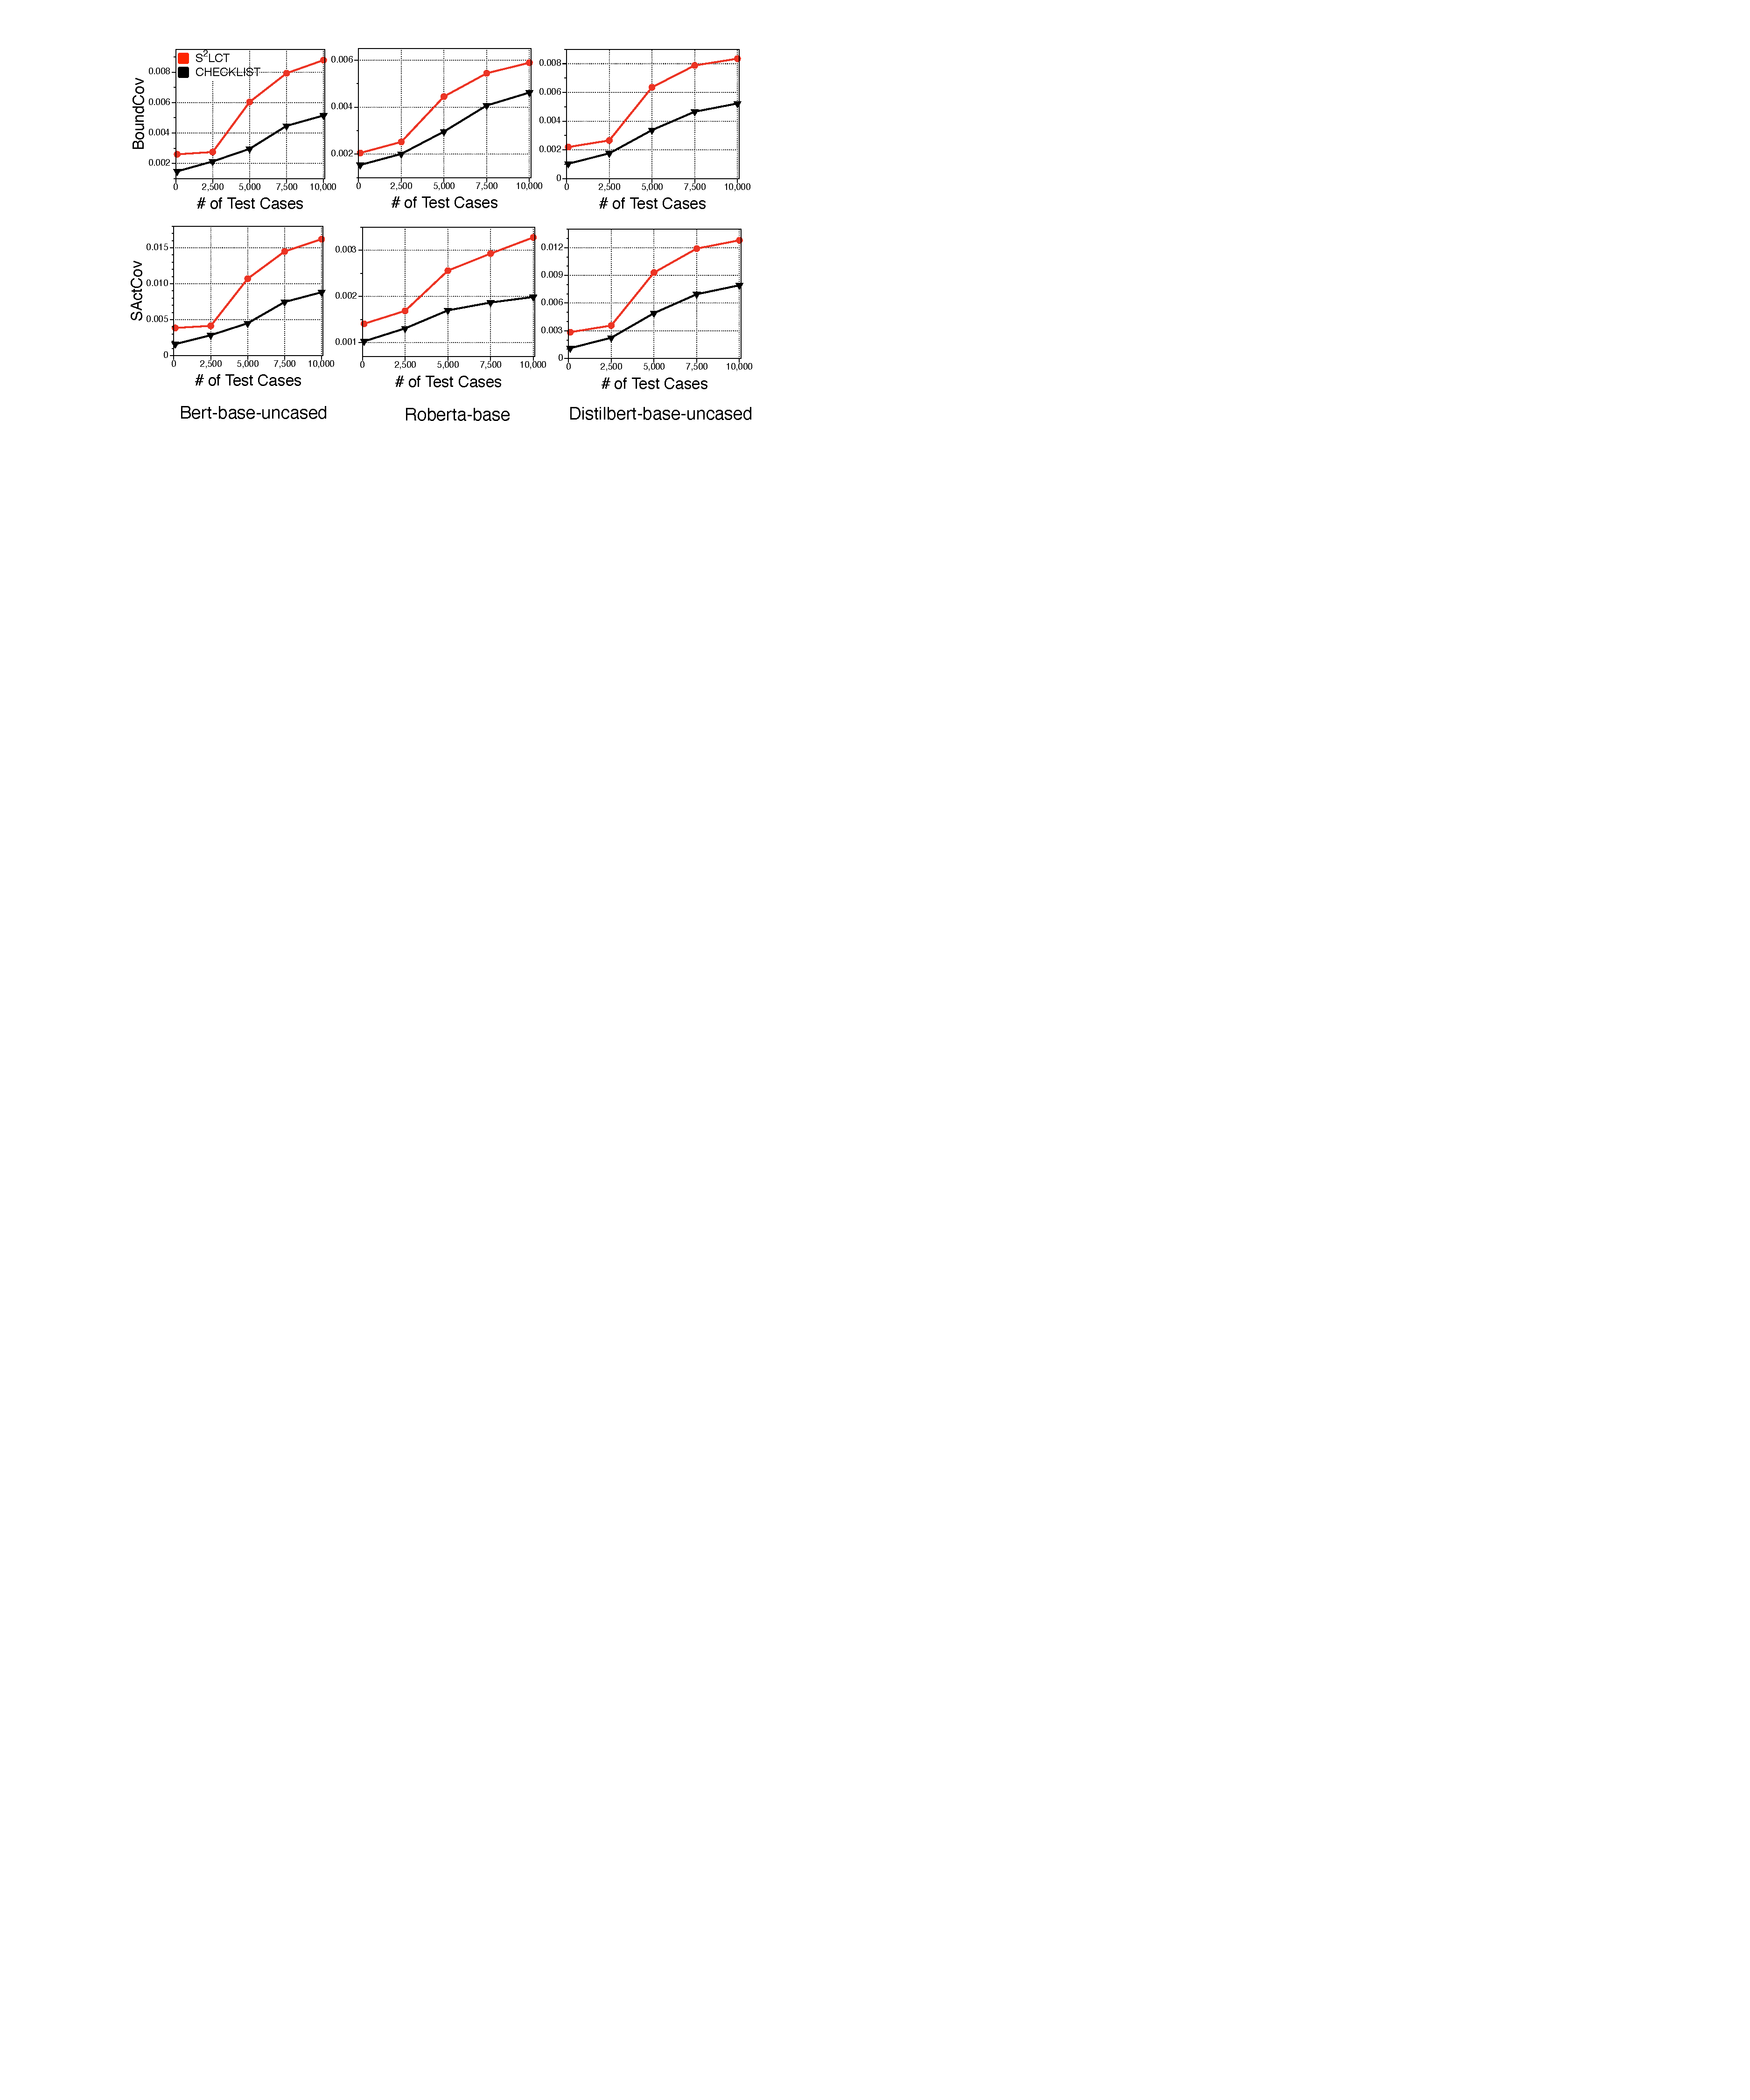
\includegraphics[width=0.5\textwidth]{figs/coverage.pdf}
    \vspace{-4mm}
    \caption{Coverage results of \tool and \Cklst test cases.}
    \label{fig:coverage}
\end{figure}

Next, Figure \ref{fig:coverage} shows the coverage results of \tool and \Cklst test cases. The red line represents \tool coverage and the black line represents \Cklst coverage. Each column in Figure \ref{fig:coverage} represents the results for one NLP model. The first row is the \textit{BoundCov} results and the second row is the \textit{SActCov} results.

We made three observations.
First, for \emph{all} experimental settings (i.e., NLP model and coverage metric), \tool achieves higher coverage than \Cklst. Recall that a higher coverage implies the test cases are more diverse and do not have a similar statistical distribution to the model training data. As a result, a test suite with greater coverage complements the model training data distribution (\ie holdout testing data) better.
For example, for the first NLP model under test, \tool can achieve a higher coverage than \Cklst with only half the number of test cases.
This result confirms that \tool can generate more diverse test cases to complement the holdout dataset for testing NLP models.

Second, as the number of test cases increases, the test suite can achieve better coverage. Such observation is intuitive. However, generating a more extensive test suite is not easy, particularly  for \Cklst, which is a manually template-based approach.

Third, for each NLP model, there is no fixed relationship between \textit{BoundCov} and \textit{SActCov}. In other words, while a test suite may produce higher \textit{BoundCov} for some models, the same test suite may get higher \textit{SActCov} for other NLP models.
Recall that \textit{BoundCov} measures both the upper and lower corner neurons and \textit{SActCov} measures only the upper corner neurons. 
Such observation implies that the upper and lower corner neurons are distributed unevenly, and measuring only one of them is not enough.

%\subsection{Explainability Case Study}

